\begin{align*}
       P &= r cos(\theta_2 - \theta)                           \\
       R &= (\theta, r)                                        \\
 \theta  &= atan2(y,x)                                         \\
       r &= \sqrt(x^2+y^2)                                     \\
       x &= r_1 \cdot cos(\theta_1)+ r_2 \cdot cos(\theta_2)               \\
       y &= r_1 \cdot sin(\theta_1)+ r_2 \cdot sin(\theta_2)               
\end{align*}
\begin{tikzpicture}[scale=2.8]
%set angles here. wall angle is what laser range scanner measures  (relative to robot)
\newcommand{\robotAngle}{30}
\newcommand{\wallAngle}{20}

                                                                                                                             %coordinate axis
\draw[->] (0,0) -- (5,0) node[right]                                                                                         {\(x_{global}\)};
\draw[->] (0,0) -- (0,5) node[above]                                                                                         {\(y_{global}\)};

%robot
\node[name=robot] at (\robotAngle:2cm) {};

                                                                                                                             %robot relative coordinate axis
\draw[rotate=\robotAngle,->] (robot.center) -- ++(3,0) node[right]                                                           {\(x_{robot}\)};
\draw[rotate=\robotAngle,->] (robot.center) -- ++(0,3) node[right]                                                           {\(y_{robot}\)};

%calculate theta_2
\FPeval{\thetaTwo}{clip(\robotAngle + \wallAngle)}        

%wall
\node[scale=0.3,fill=black, minimum width=15cm, rotate={90 + \robotAngle + \wallAngle}, name=wall] at ([shift=(\thetaTwo:2cm)] robot.center) {};
\node[name=midwall] at ($(wall.180)!(robot.center)!(wall.0)$) {};
\node[above] at (wall.0) {wall};

                                                                                                                             %laser range output
\draw[very thick, red]  (midwall.center) -- (robot.center) node[black,midway, left]                                          {\(r\)};
\draw[very thick, red]   ([shift=(\robotAngle:1cm)] robot.center) arc(\robotAngle:\thetaTwo:1cm) node[near end, black,right] {\(\theta_{wall}\)};

                                                                                                                             %robot position
\draw[dashed] (robot.center) -- ++(3,0) node[right]                                                                          {\tiny\( 0\degree\)};
\draw[dashed] (robot.center) -- ++(0,3) node[above]                                                                          {\tiny\(\frac{\pi}{2}\degree\)};
\draw[very thick, green] ([shift=(\robotAngle:1cm)] robot.center) arc(\robotAngle:0:1cm)  node[midway, black,right]          {\(\alpha\)};

                                                                                                                             %summated vector of robot and wall angle
\path (midwall); \pgfgetlastxy{\XCoord}{\YCoord};
\draw[very thick, dashed, green] (0,0) -- (midwall) node[black, midway, left]                                                {\(r_1\)};
\draw[very thick, green] (0.5,0) arc(0:{atan(\YCoord/\XCoord)}:0.5cm) node[midway, black, right]                             {\(\theta\)};
                                                                                                                             
                                                                                                                             %real angle to wall                                                                                                          
\node[name=projected] at ($(wall.180)!(0,0)!(wall.0)$) {};                                                                   
\draw[very thick, dashed,blue] (projected.center) -- (0,0) node[black, midway, left]                                         {\(r_2\)};
\draw[very thick, blue] (1.5,0) arc(0:\thetaTwo:1.5cm) node[midway, black,right]                                             {\(\theta_2\)};

                                                                                                                             %I am not sure what we use this angle for...
\draw[dashed,red!50] (0,0) -- (robot.center) ;
\draw[very thick,red!50] ([shift=(\robotAngle:1cm)] (0,0) arc(\robotAngle:0:1cm) node[midway,black,right]                    {\(\theta_1\)};

\end{tikzpicture}

% \clearpage
% \begin{figure}
% \centering
% \begin{tikzpicture}
% 
% \draw[dashed] (-5,0) node[left] {\(\frac{\pi}{2}\)} -- (5,0) node[right] {\(\frac{3\pi}{2}\)};
% \draw[dashed] (0,-5) -- (0,5) node[above] {\(0\)};
% 
% \node[name=robot] at (0,0) {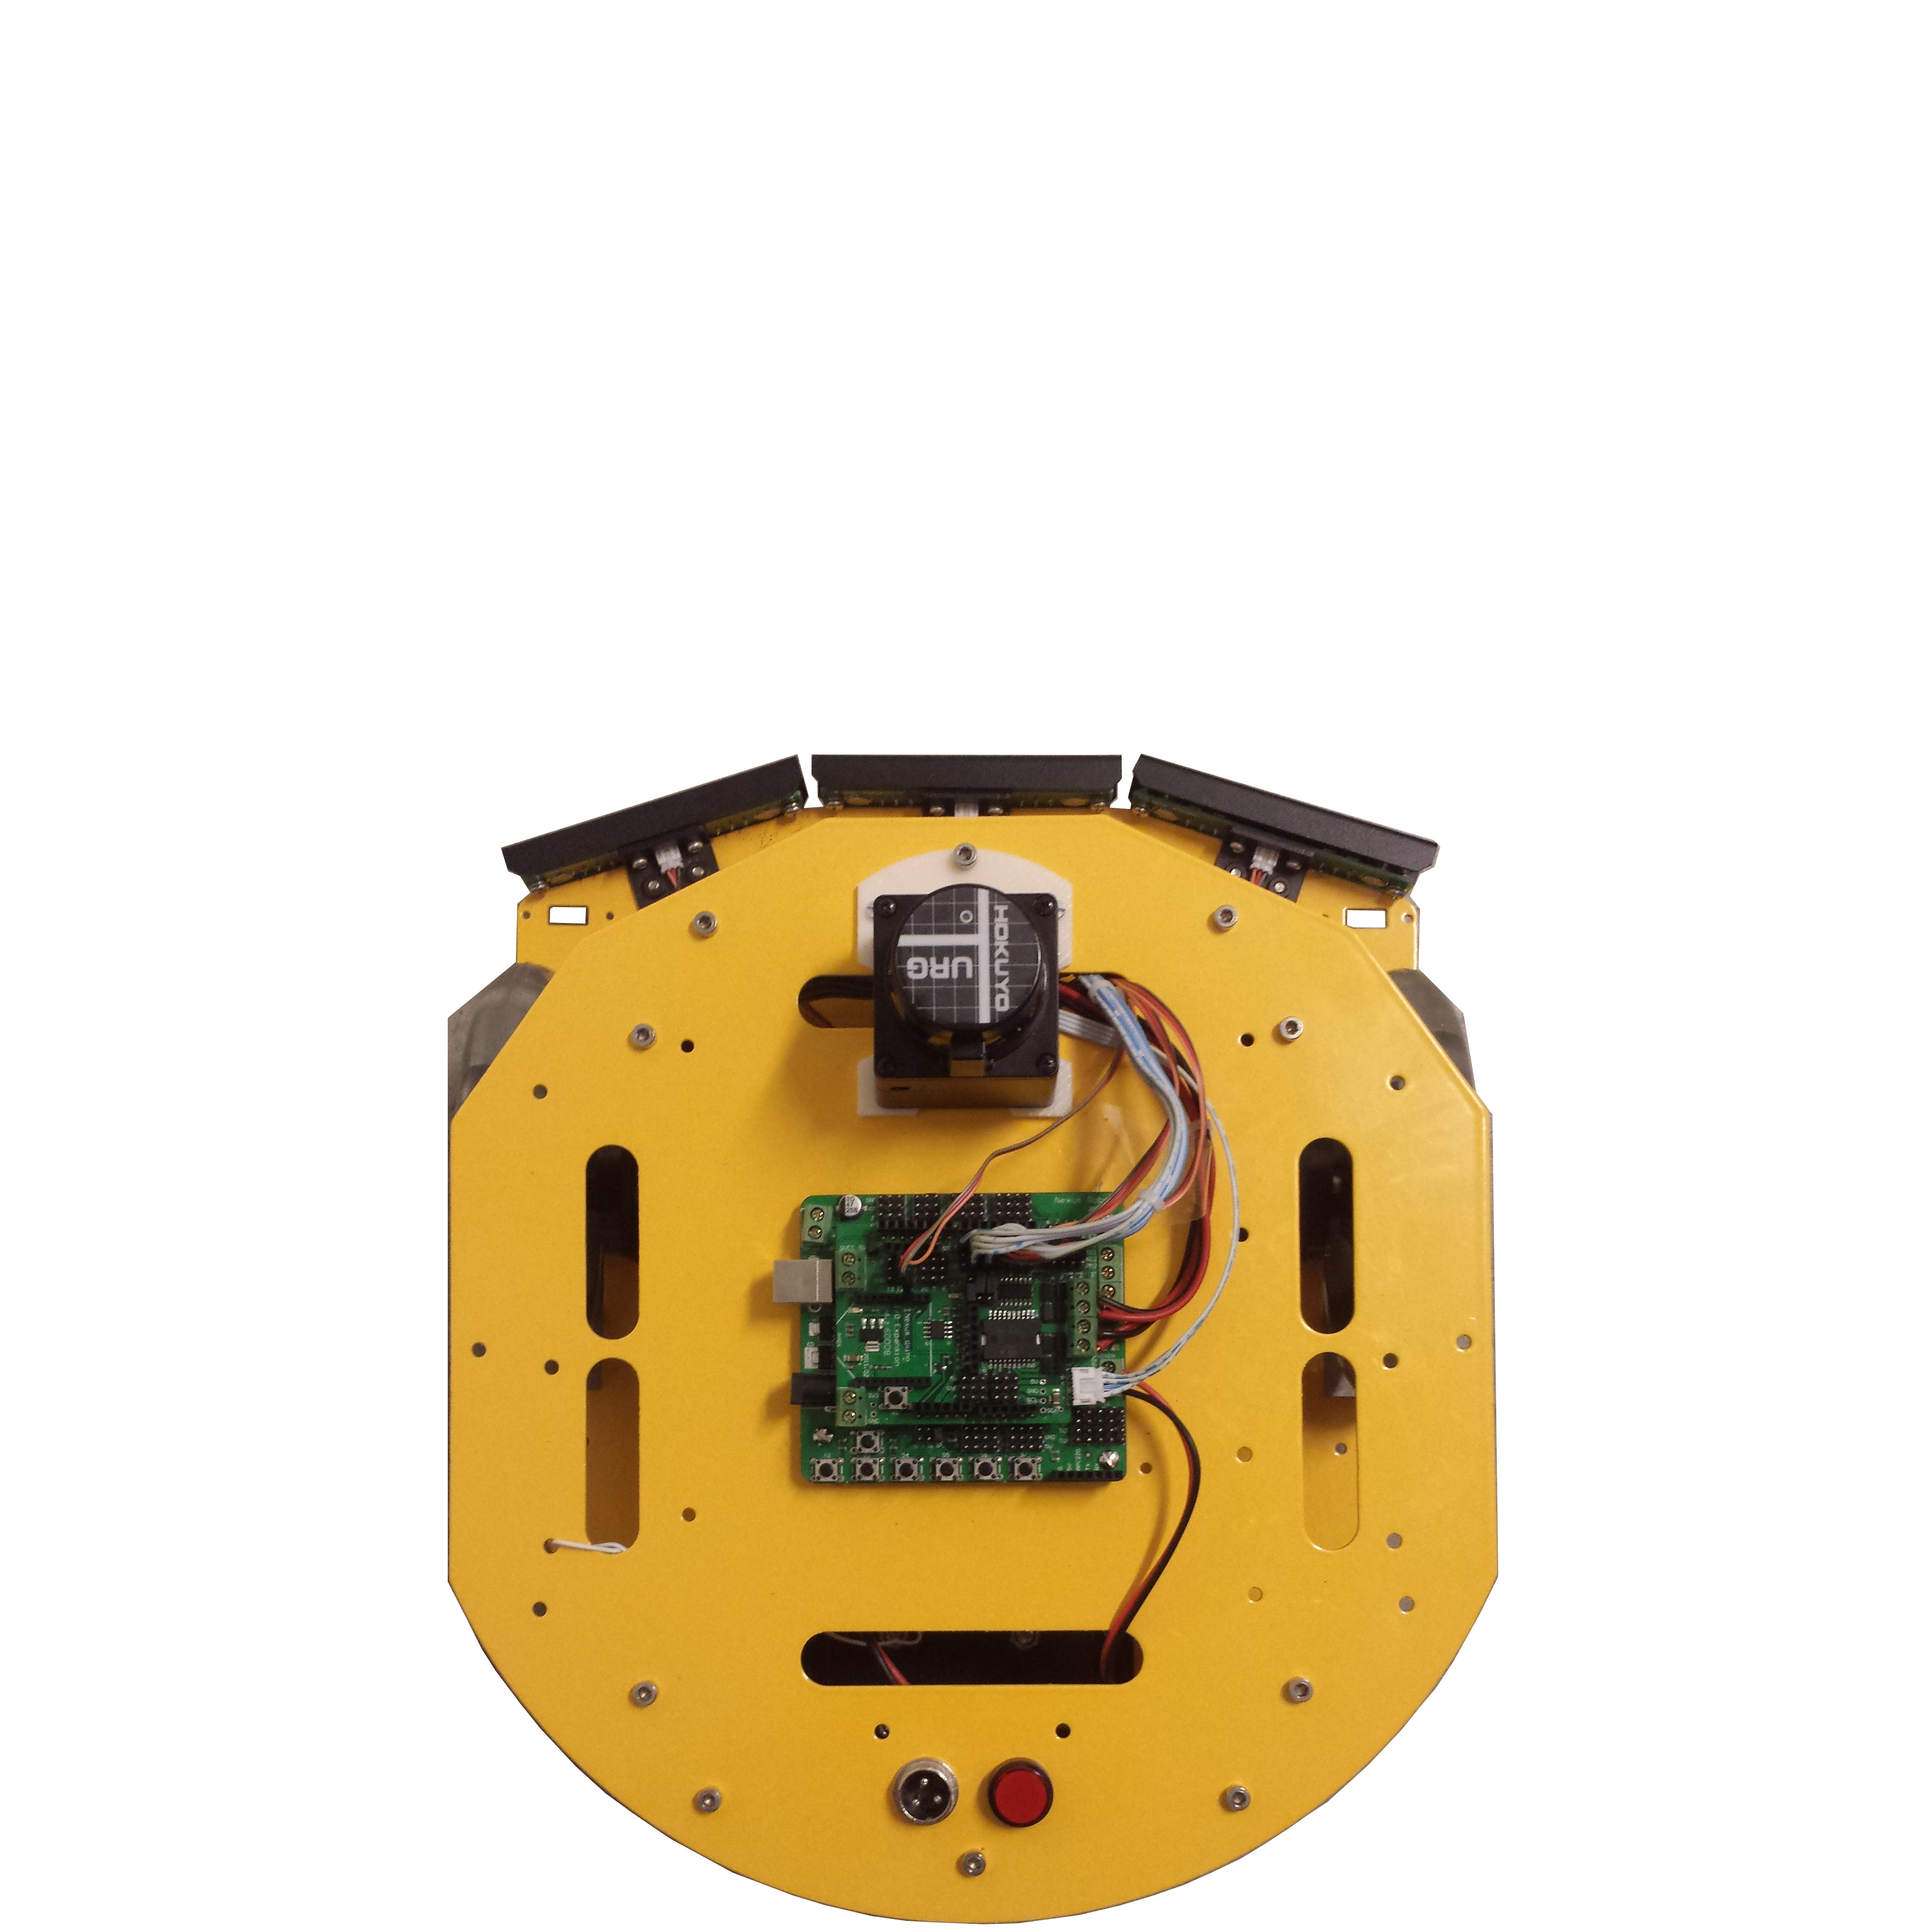
\includegraphics[width=5cm]{graphics/robot2}};
% \fill[pattern color=gray!50, pattern=crosshatch]  (robot.center) -- (210:5cm) arc(210:330:5cm);
% \fill[pattern color=red!50,  pattern=crosshatch]  (robot.center) -- (330:5cm) arc(-30:210:5cm);
% 
% \end{tikzpicture}
% \end{figure}

